\RequirePackage{ifpdf}
\ifpdf
	\documentclass[11pt,oneside,a4paper,pdftex]{article}   %two-page printing
\else
	\documentclass[11pt,twoside,a4paper,dvips]{article}   %two-page printing
\fi

%\documentclass[a4paper, 12pt]{article}
\addtolength{\hoffset}{-1.9cm}
\addtolength{\voffset}{-1.9cm}
\addtolength{\textwidth}{+3.8cm}
\addtolength{\textheight}{+3.8cm}
\usepackage[latin1,utf8]{inputenc}
\usepackage[czech]{babel}
\usepackage{icomma} % ceska desetinna carka
\usepackage{listings}
\usepackage{amsmath}
\usepackage{amsthm}
\usepackage{amsfonts}
\usepackage{mathrsfs}
%\usepackage[T1]{fontenc}
\ifpdf
	\usepackage[pdftex]{graphicx} % dvips or pdftex
\else
	\usepackage[dvips]{graphicx} % dvips or pdftex
\fi
\usepackage[center]{subfigure}
\usepackage{amsfonts}
%\usepackage[small,hang]{caption2}      %figure caption
\usepackage[dvips]{color}               %for using colors
%\usepackage{showframe}                 %zobrazuje okraje stranky
\usepackage[justification=centering]{caption}
\usepackage{textpos}
\usepackage{url}
%\usepackage{fancybox}
\usepackage{verbatim}
\usepackage{fj}
\ifpdf
	\usepackage[pdftex,unicode,colorlinks]{hyperref}
\else
	\usepackage[unicode]{hyperref}
\fi


%FIXME: odlišit font, aby části kódu byly odlišitelné od okolního textu
\lstset{ %
language=Matlab,           % choose the language of the code
basicstyle=\ttfamily,   % the size of the fonts that are used for the code
numbers=none,             % where to put the line-numbers (none, left, ..)
numberstyle=\scriptsize,  % size of the fonts used for the line-numbers
stepnumber=1,             % step between two line-nums. If "1" each line nmbrd
numbersep=10pt,            % how far the line-numbers are from the code
%backgroundcolor=\color{white},
	% choose the background color. You must add \usepackage{color}
showspaces=false,         % show spaces adding particular underscores
showstringspaces=false,   % underline spaces within strings
showtabs=false,           % show tabs within strings
frame=none,	          % adds a frame around the code (single, none, ...)
tabsize=2,	          % sets default tabsize to 2 spaces
captionpos=b,             % sets the caption-position to bottom
breaklines=false,          % sets automatic line breaking
breakatwhitespace=true,   % sets if automatic breaks should only happen at \s
%escapeinside={\%*}{*)}   % if you want to add a comment within your code
}

\title{Domácí úkol, A3M33PRO 2011 - Pokročilá robotika - HW-04}
\date{16. 10. 2011}
\author{Filip Jareš}

\begin{document}

\maketitle

\section{Zadání}

\begin{enumerate}
\item Zkonstruujte popis robotu Mitsubishi Melfa RV-6 v Denvit-Hartenberg konvenci na
základě návodu Denavit-Hartenberg.pdf a podle dokumentace MELFA-RV-6S.
\item Implementujte simulátor robotu v MATLAB Robotic Toolbox.
Robotický toolbox po rozbalení přidáte do cesty:
\begin{lstlisting}
addpath('robot');
L{1} = link([alpha, a, 0, d, 0, theta_offset ],'standard');
L{2} = ...
\end{lstlisting}
Robota (s rotačními klouby) vytvoříte pomocí příkazu:
\begin{lstlisting}
r = robot(L, 'PRO', 'name', '');
\end{lstlisting}
Robota zobrazíte pomocí příkazu (vzorový výstup):
\begin{lstlisting}
drivebot(r);
view([1;1;1]);
\end{lstlisting}
\end{enumerate}

\noindent Vypracovanou úlohu tvoří zip soubor obsahující:

\begin{enumerate}
   \item \lstinline{dhsim.m} - implementace simulátoru v MATLAB Robotic Toolboxu.
   \item \lstinline{dh.pdf} - dokument obsahjící:
		\begin{enumerate}
				\item Nákres os pohybu a zvolených souřadných soustav, včetně označení a očíslování a vyznačených orientací úhlů.
				\item DH parametry všech os.
				\item Popis konstrukce souřadných soustav a zdůvodnění všech možných voleb.
				\item Popis implementace v MATLAB Robotic Toolboxu.
		\end{enumerate}
\end{enumerate}

\newpage
\section{Popis robotu v D-H konvenci}

\noindent Uspořádání robotu Mitsubishi Melfa RV-6 je znázorněno na \figref{fig:foto}. Počátek světového souřadného systému
byl umístěn do průsečiku kloubů J1 a J2 s osou $x$ směřující na \figref{fig:foto} téměř směrem k po\-zo\-ro\-va\-te\-li
a osou $z$ směrující nahoru. Nákres os pohybu a zvolených souřadných soustav pro konstrukci popisu
robotu v Denavit-Hartenbergově konvenci je zná\-zo\-rněn na \figref{fig:soustavy}. Výkres, ze kterého
byly odečteny potřebné rozměry robotu je na \figref{fig:vykres}. U~souřadných
soustav jednotlivých kloubů bylo při volbě orientace os $z$ (které představují osy kloubů)
přihlédnuto k orientacím úhlů zavedeným pro jednotlivé klouby na \figref{fig:foto}.
Výsledné D-H parametry všech os jsou shrnuty v tabulce \ref{tab:DH_parametry}.

Získaný popis robotu pomocí D-H parametrů byl použit k vytvoření modelu robotu s~využitím Matlab Robotics Toolboxu.
Model ve dvou konfiguracích je znázorněn na \figref{fig:robot_toolbox}.

Aktuální verze Matlab Robotics Toolboxu má oproti verzi použité v zadání změněné názvy
některých funkcí.

\begin{figure}[htb]
	\centering
	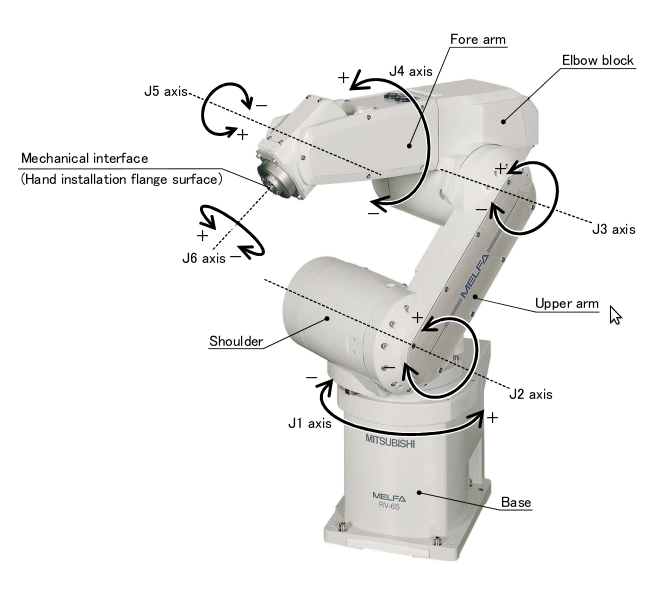
\includegraphics[width=15.3cm]{pictures/picture-Mitsubishi-Melfa-RV-6S-s_popisky.png}
	\caption{Fotografie robotu s označením jednotlivých os a orientací úhlů}
	\label{fig:foto}
\end{figure}

\begin{figure}[htb]
	\centering
	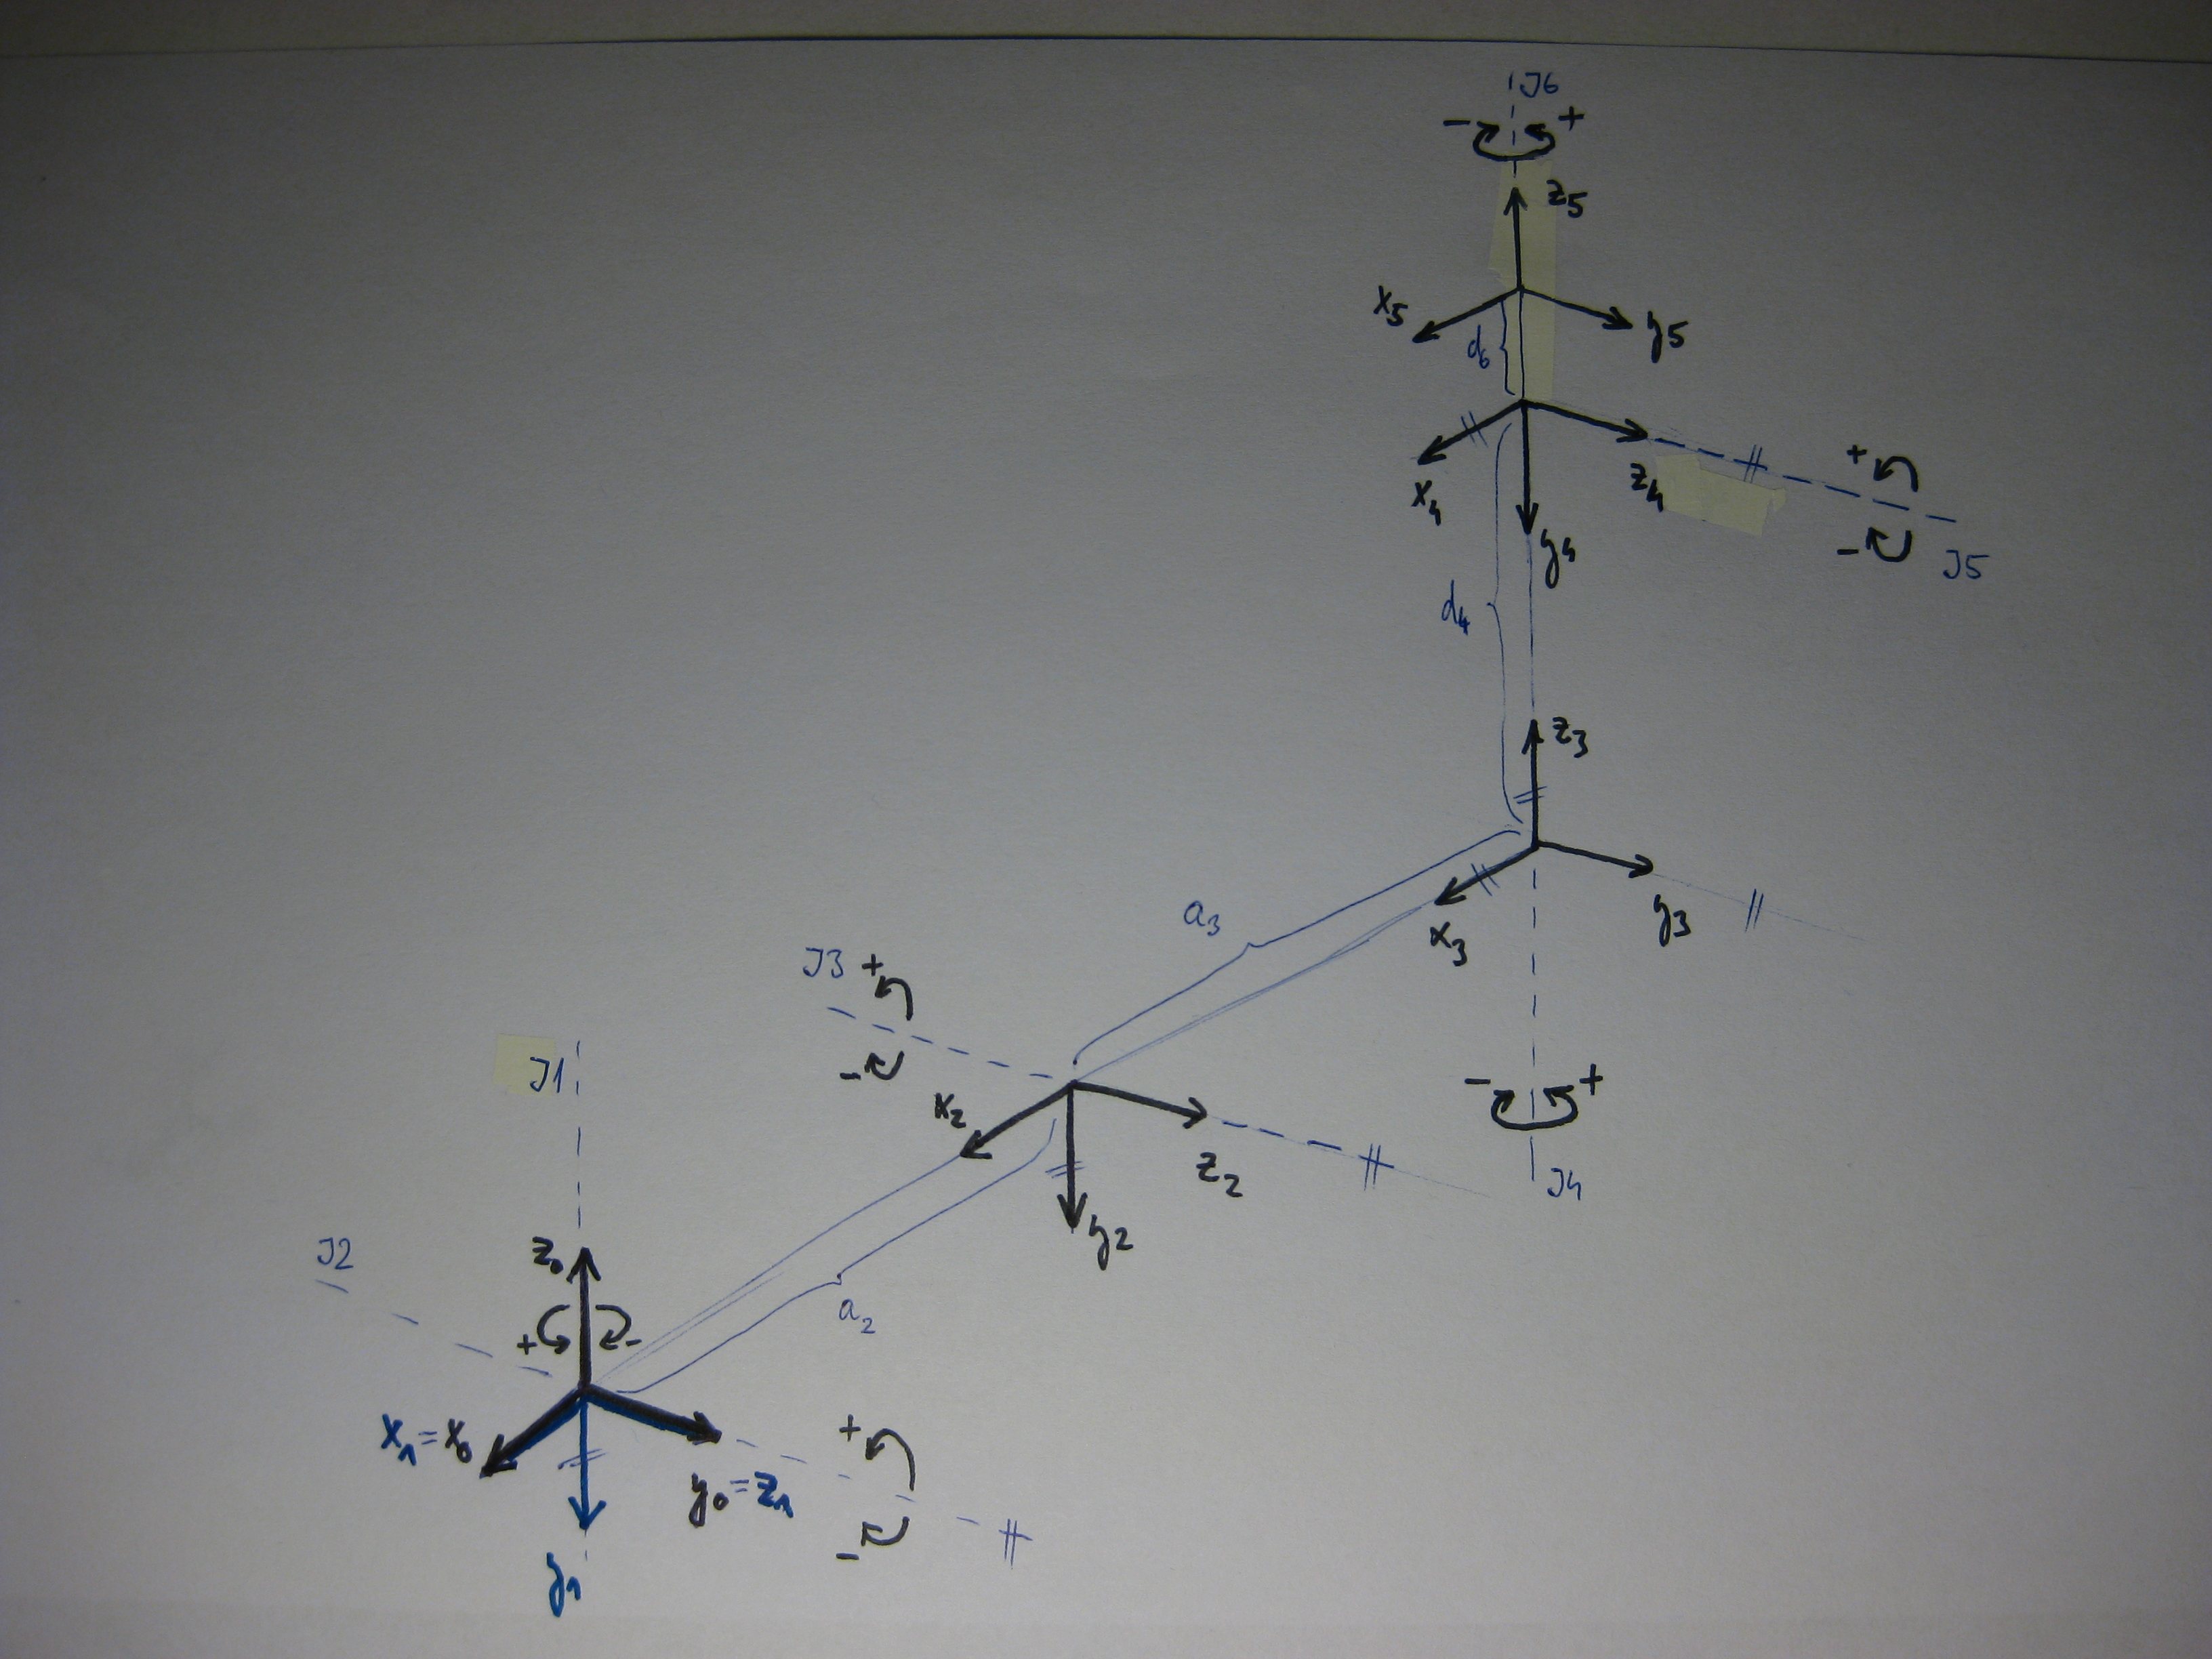
\includegraphics[width=15.3cm]{pictures/img_5916.jpg}
	\caption{Nákres os pohybu (J1 až J6) a zvolených souřadných soustav}
	\label{fig:soustavy}
\end{figure}


\begin{table}[htb]
	\centering
	\begin{tabular}{|c|c|r|r|r|}
		\hline
		$i$	& $\theta_i$ (rad)	& $d_i$ (m)				& $a_i$	(m)			& $\alpha_i$ (rad)\\
		\hline
		1	& $q_1$				& 0\phantom{,000}		& 0\phantom{,000}	& $-\pi/2$	\\
		2	& $q_2$				& 0\phantom{,000}     	&-0,280				& 0			\\
		3	& $q_3$				& 0\phantom{,000}     	&-0,1\phantom{00}	& $\pi/2$	\\
		4	& $q_4$				& 0,315					& 0\phantom{,000}	& $-\pi/2$	\\
		5	& $q_5$				& 0\phantom{,000}     	& 0\phantom{,000}  	& $\pi/2$	\\
		6	& $q_6$				& 0,085					& 0\phantom{,000}  	& 0			\\
		\hline
	\end{tabular}
	\caption{Denavit-Hartenbergovy parametry jednotlivých os robotu Mitsubishi Melfa RV-6}
	\label{tab:DH_parametry}
\end{table}

\begin{figure}[htb]
	\centering
	\subfigure[Robot v konfiguraci s \uv{nulovými} úhly; vektor úhlů $q_z = (0,\ 0,\ 0,\ 0,\ 0,\ 0)$] {
		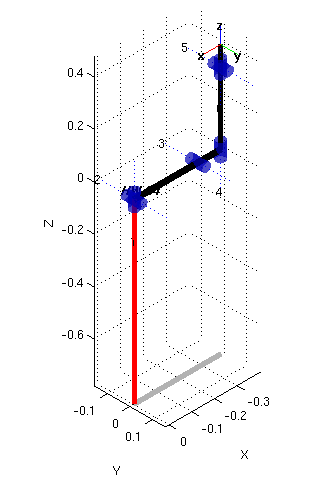
\includegraphics[width=6.5cm]{pictures/picture-robotic_toolbox_zero_configuration.png}
		\label{fig:qz}
	}
	\subfigure[Robot v konfiguraci dané vektorem úhlů $q_r = (0,\ \pi/3,\ \pi/6,\ 0,\ \pi/4,\ 0)$] {
		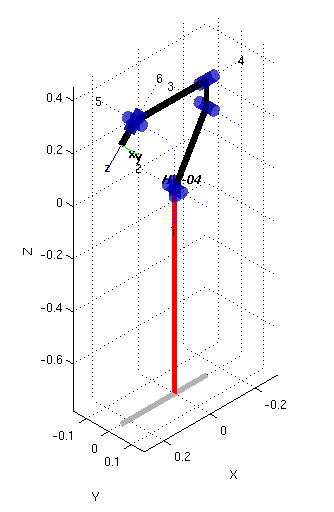
\includegraphics[width=6.5cm]{pictures/picture-robotic_toolbox_ready_configuration.png}
		\label{fig:qr}
	}
	\caption{Dvě konfigurace modelu robotu v Matlab Robotic Toolboxu}
	\label{fig:robot_toolbox}
\end{figure}

\begin{figure}[htb]
	\centering
	\fbox{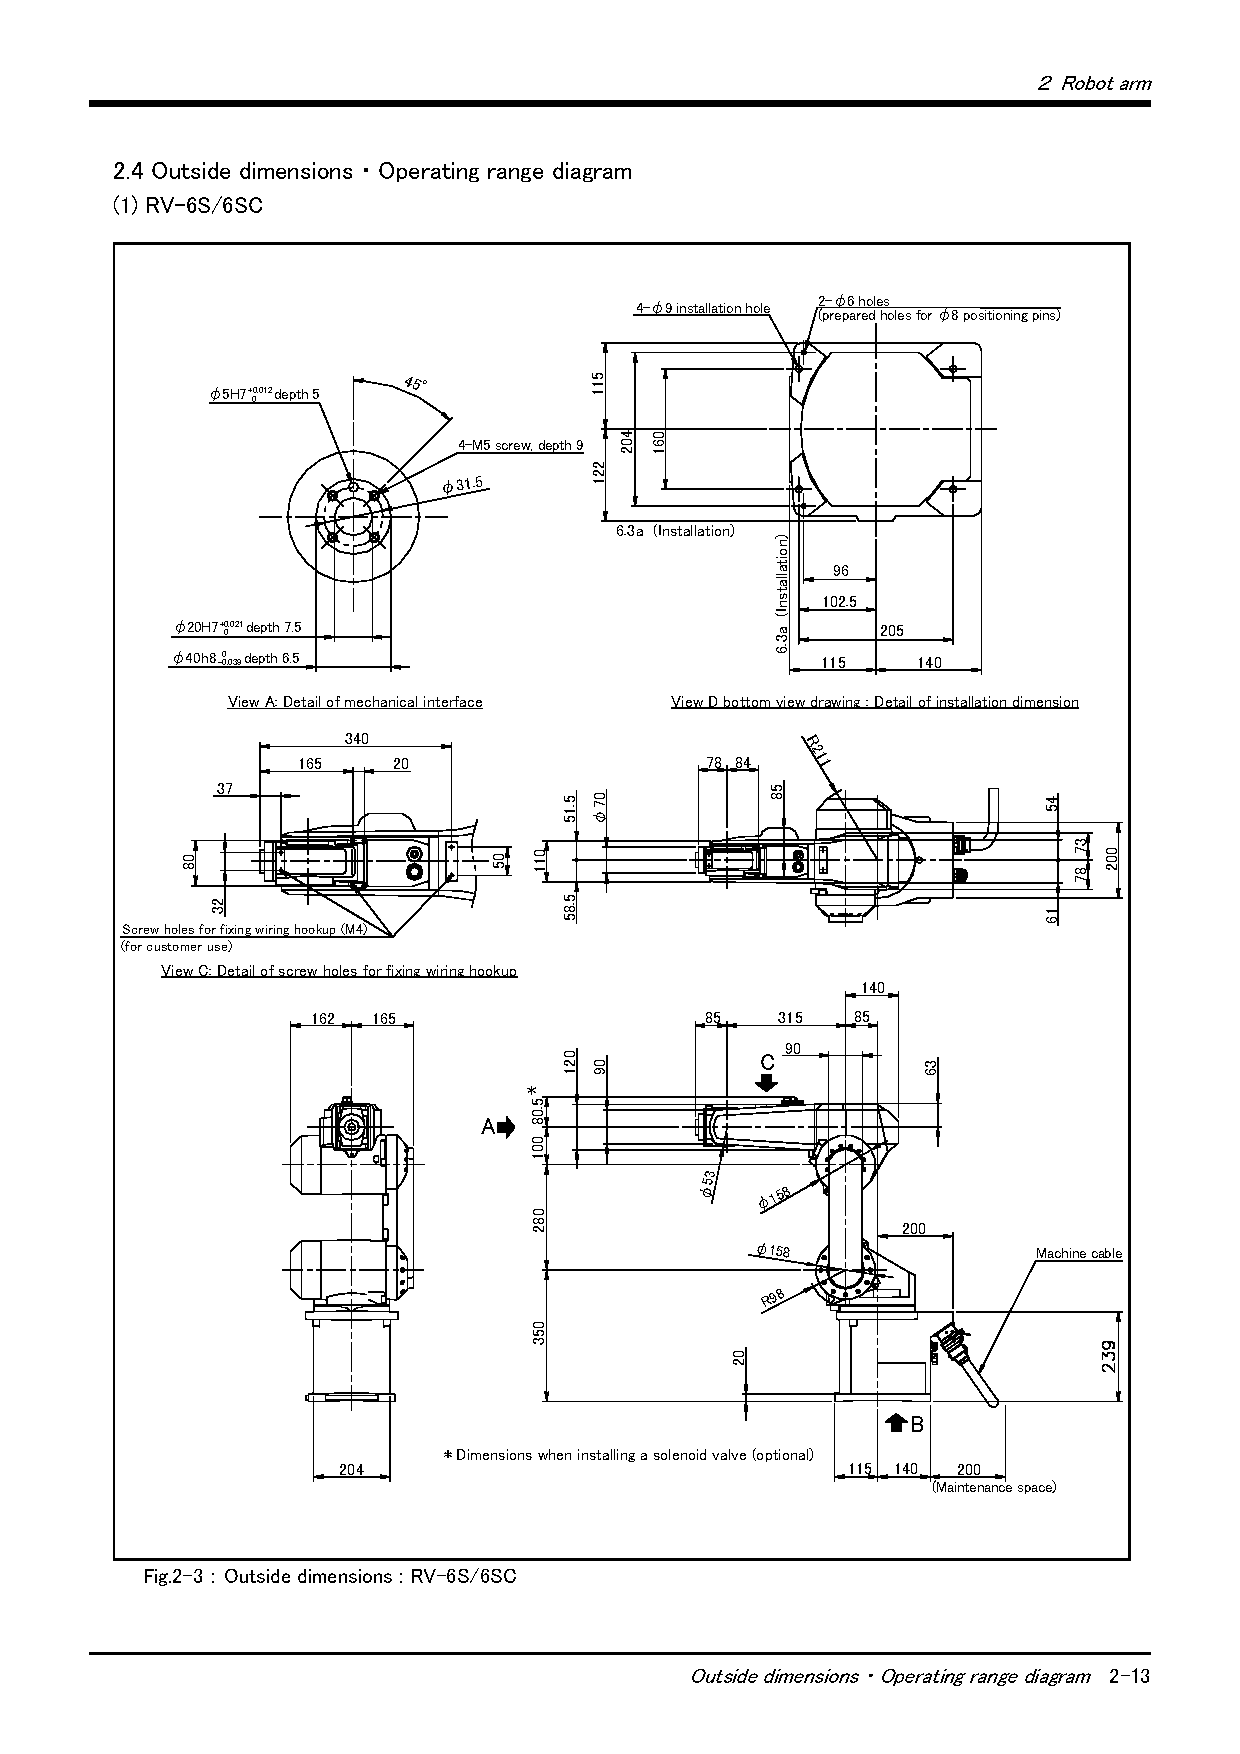
\includegraphics[width=14cm]{Mitsubishi-Melfa-RV-6S-page-0021.pdf}}
	\caption{Stránka z manuálu s kótovaným výkresem robotu}
	\label{fig:vykres}
\end{figure}

% The Bibliography
%\bibliographystyle{plain_cz}
%\bibliographystyle{czechiso}
%\bibliography{bibliography}

\end{document}

